\documentclass[a4paper,9pt]{ltjsarticle}
\usepackage{graphicx}
\usepackage{luatexja-fontspec}
\usepackage{caption}
\usepackage{amsmath,amssymb,bm,braket}
\usepackage[english]{babel}
\usepackage{multicol}
\usepackage{titlesec}
%\usepackage{gnuplot-lua-tikz}
\usepackage[top=20truemm,bottom=20truemm,left=20truemm,right=20truemm]{geometry}
\usepackage{array}
\usepackage{upgreek}
\usepackage{fancyhdr}
\renewcommand{\refname}{}
\usepackage{listings,jvlisting}
\usepackage{tikz}
\usepackage[thmmarks,amsmath]{ntheorem}
\usepackage[version=3]{mhchem}
\usetikzlibrary{external}
\tikzexternalize
\lstset{
  basicstyle={\ttfamily},
  identifierstyle={\small},
  commentstyle={\smallitshape},
  keywordstyle={\small\bfseries},
  ndkeywordstyle={\small},
  stringstyle={\small\ttfamily},
  frame={tb},
  breaklines=true,
  columns=[l]{fullflexible},
  numbers=left,
  xrightmargin=0pt,
  xleftmargin=3pt,
  numberstyle={\scriptsize},
  stepnumber=1,
  numbersep=1pt,
  lineskip=-0.5ex
}
\captionsetup[figure]{format=plain, labelformat=simple, labelsep=quad,labelfont=bf,name={Fig.}}
\captionsetup[table]{format=plain, labelformat=simple, labelsep=quad,labelfont=bf}
\parindent = 0pt
%[BoldFont=HGSMinchoE]{MSMincho}[BoldFont=HiraMinProN-W6]{HiraMinPro-W3}
\titleformat{\section}{\normalfont\fontsize{9}{10}\bfseries\fontspec{Times New Roman}}{\thesection.}{1em}{}
\usepackage[backend=biber,sorting=none,style=numeric,maxnames=99,minnames=1]{biblatex}
\addbibresource{utility/REFERENCES.bib}
\defbibheading{bibliography}[\refname]{%
  \section*{REFERENCES}%
  \vspace{-7pt}  % ここで空白を調整。お好みの値に変更してください。
}
\newfontfamily\subsectionfont{Times New Roman} % サブセクション用フォント
\titleformat{\subsection}
  {\normalfont\large\bfseries} % サブセクションのフォントを指定
  {\thesubsection}{1em}{}
\renewbibmacro{in:}{}
\renewbibmacro*{journal+issuetitle}{%
  \addcomma\space% カンマとスペースを追加
  \usebibmacro{journal}%
  \setunit*{\addspace}%
  \usebibmacro{volume+number+eid}%
  \setunit{\addspace}%
  \printfield{note}%
  \newunit
}
\renewbibmacro*{volume+number+eid}{
  \printfield{volume}%
  \setunit*{\addnbspace}%
  \printfield{number}%
  \setunit{\addcomma\space}%
  \printfield{eid}
}
\DeclareFieldFormat[article]{volume}{\textbf{#1}}
\DeclareFieldFormat[article]{pages}{#1}
\DeclareFieldFormat{journaltitle}{#1}
\usepackage{hyperref}
\renewenvironment{abstract}{\par\noindent}{\par}
%\pagenumbering{gobble}
\usepackage{docmute}
\usepackage{setspace}
\usepackage{titlesec} % 見出しのカスタマイズ用

% セクションのフォーマットをカスタマイズ
\titleformat{\section}
  {} % フォントサイズとスタイル
  {\Large\bfseries\thesection\ \ }               % 番号の前の内容(空白)
  {0em}            % 番号とタイトルの間の間隔
  {\Large\bfseries}


\theoremstyle{plain}
\theoremheaderfont{\normalfont\bfseries}
\theorembodyfont{\itshape}   % 本文を斜体に
\theoremseparator{.}         % タイトルと本文の区切りを「.」に設定
\newtheorem{definition}{Definition}
\begin{document}
\centerline{\Large\bfseries Floquet Color Codeについて}
\vspace{10pt}
 \cite{kesselring2024}に示されている、Floquet Color Codeについてどのような性質があるのか調べてみた。
\section{Color Code}
   Color Code(CC)はFig.1に示されるようなもので、六角形を平面上にならべ、隣り合う六角形の面は異なる色で塗ったものである。量子ビットは六角形格子の点の上に配置する。スタビライザー$s$はそれぞれの色の面に対応していて、色を$c$、面を$p$とすると、以下の式で表される。
  \begin{align}
    s_{c,p}^x=\prod_{j\in\mathrm{vert}(p)}X_j,\  s_{c,p}^z=\prod_{j\in\mathrm{vert}(p)}Z_j,
  \end{align}
  ここで、vert$(p)$は$p$面に属する点(角)に対応する。Fig.1の例だと、量子ビットが37個、スタビライザーが36個で、1量子ビットをエンコードできることがわかる。
  \begin{figure}[h]
    \centering
    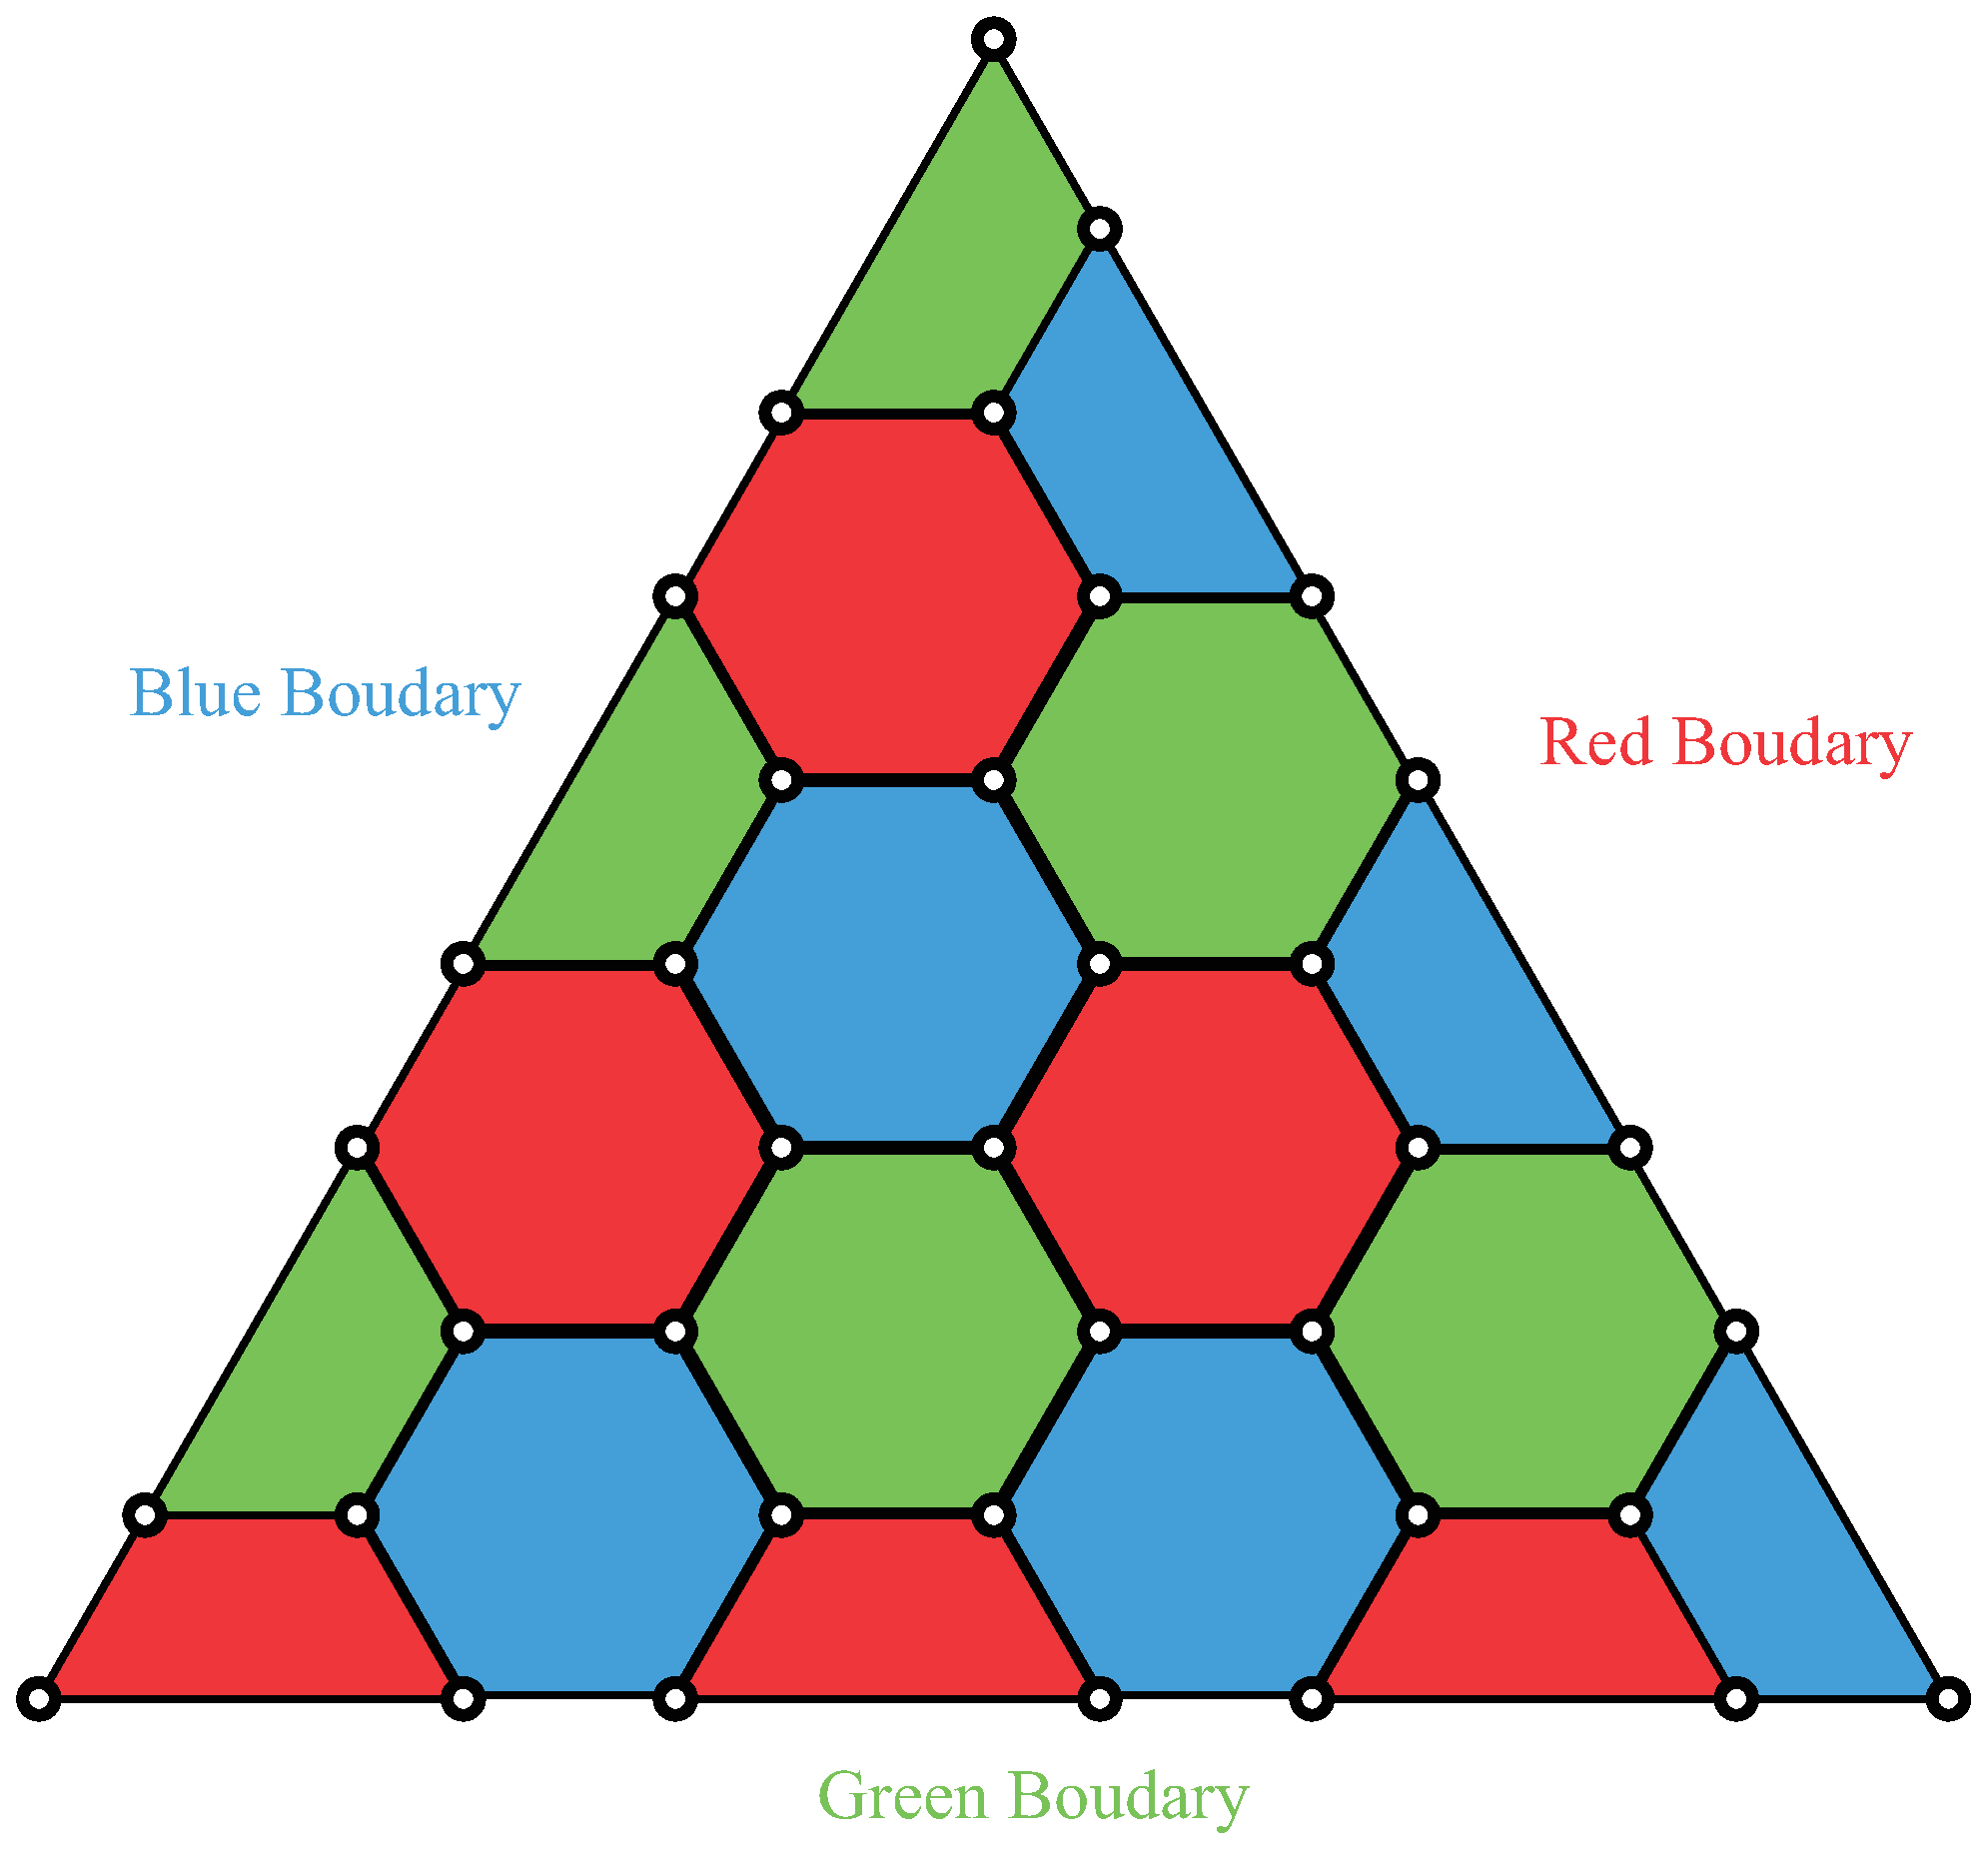
\includegraphics[scale=0.20]{figure/figure1.eps}
    \vspace{-5pt}\caption{}
    \label{figure1}
    \vspace{-15pt}
  \end{figure}\\
  また、これらのスタビライザーをハミルトニアンとして、
  \begin{align}
    H_{CC}=-\sum_{c,p}s_{c,p}^x-\sum_{c,p}s_{c,p}^z
  \end{align}
  というふうに書くとエラーが生じている状態をexitationとして、anyon粒子を構成する事ができる。赤、緑、青をそれぞれr,g,bと表すと、c面のxスタビライザーがexiteしたときはcxという粒子、c面のzスタビライザーがexiteしたときはczという粒子、c面のxとzスタビライザーがexiteしたときはcyという粒子というふうに(cにはr,g,bのどれかが入る)、9つのanyon粒子を定義することができ、それを表にしてTab.1に示す。\\
    
  \begin{table}[h]
    \centering
    \begin{tabular}{c|c|c|c}
       & r & g & b \\
      \hline
      x & rx & gx & bx \\
      \hline
      y & ry & gy & by \\
      \hline
      z & rz & gz & bz \\
      \hline
    \end{tabular}
    \caption{}
  \end{table}

  Fig.1のboudaryはこのanyon粒子のうち、どれがcondenseされるかに基づいている。ただし、説明が長くなるので具体的な性質については\cite{kesselring2024}\cite{kesselring2018}を参照。\\
   このようなanyon modelはToric Code(TC)にも適用でき、Xスタビライザーのexitationをe粒子、Zスタビライザーのexitationをm粒子として表す。また、eはsmooth boudaryでcondenseされ、mはrough boundaryでcondenseされる。
\clearpage
\section{Floquet Color Code}
   Floquet Color CodeはFig.1のCCで、一つの色とPauliを選んで、Fig.2のようにスタビライザーを選んだものである。ここで、赤線は2-weightのXスタビライザー、赤字Xの面は6-weightのXスタビライザー、青と緑の面は6-weightのZスタビライザーである。境界のスタビライザーは、扇形に属する点へのXまたはZスタビライザーである(おそらく)。また、境界にある赤点は2-weightのXスタビライザー(赤線)が1-weightになったものである。おそらくこの例では、符号距離が8である。
  \begin{figure}[h]
    \centering
    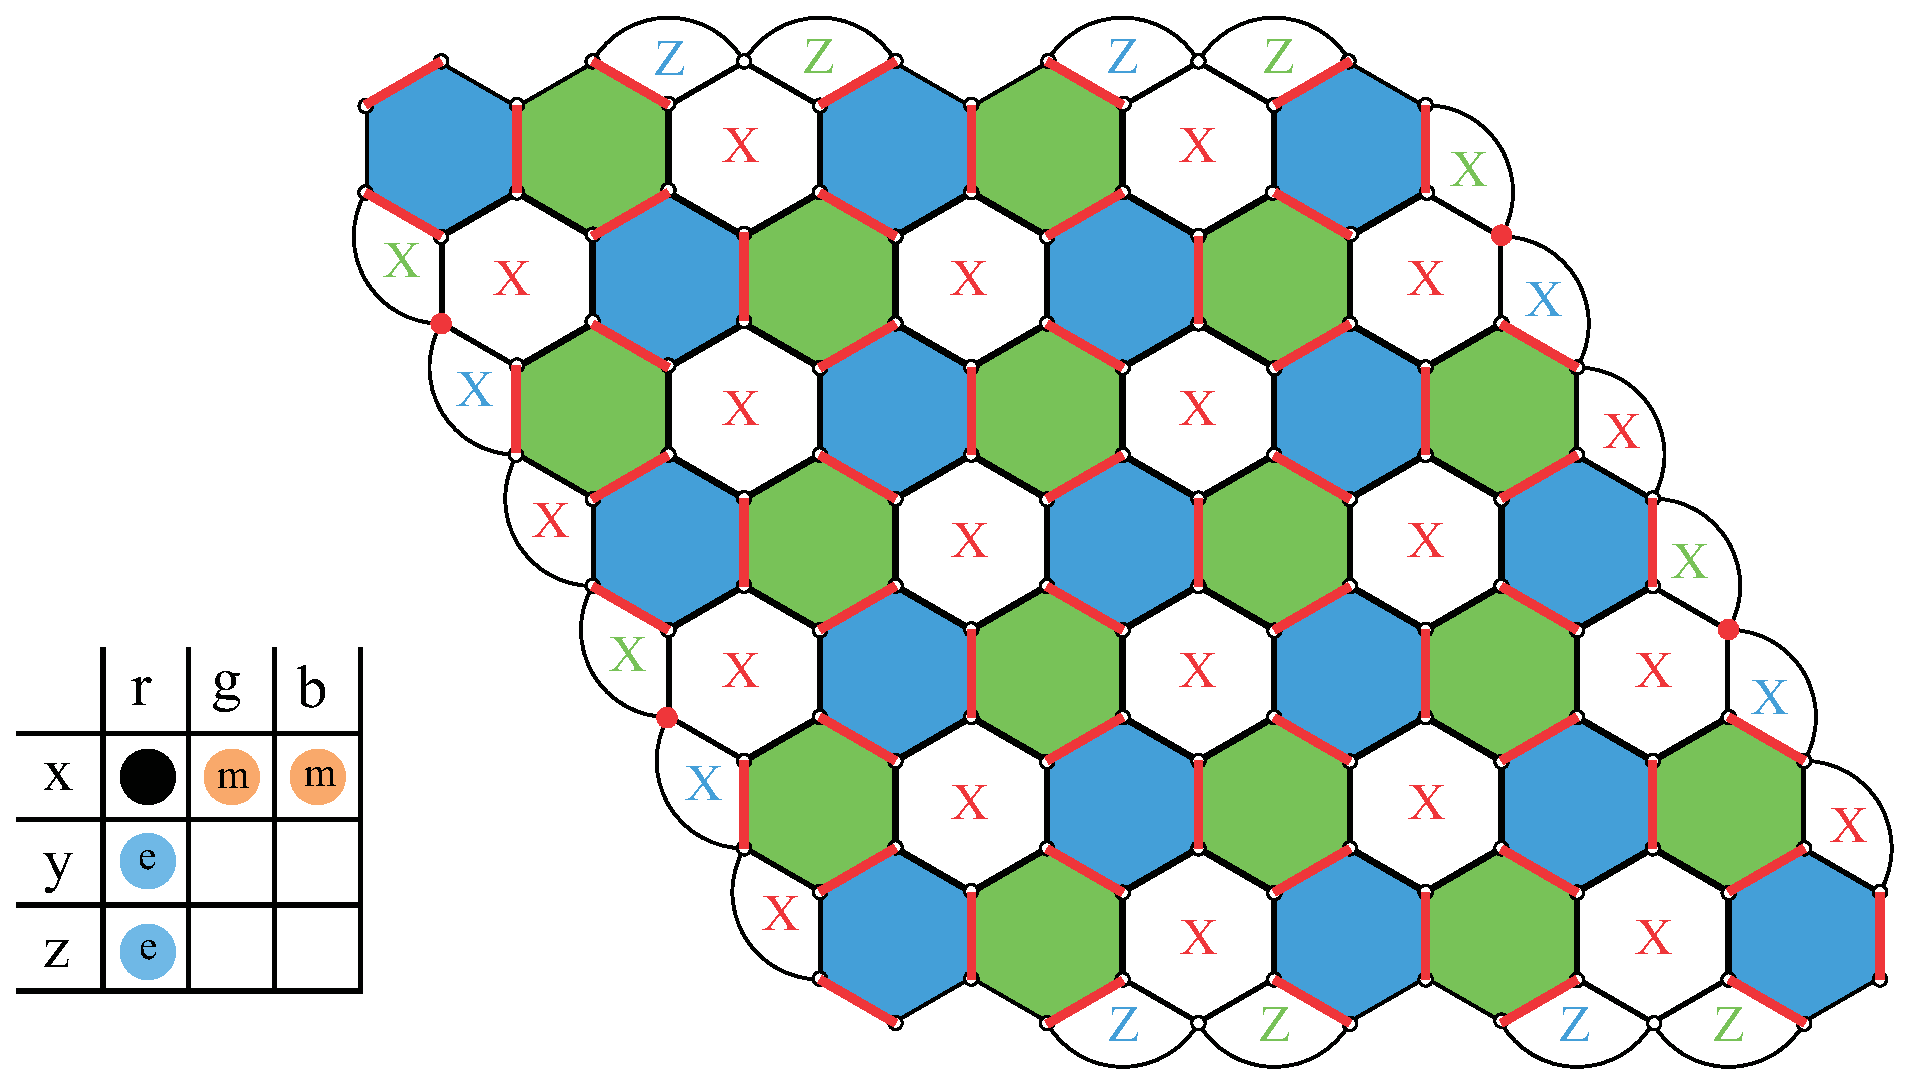
\includegraphics[scale=0.30]{figure/figure2.eps}
    \vspace{10pt}\caption{}
    \label{figure2}
    \vspace{-15pt}
  \end{figure}\\
  Fig.2の例が\cite{kesselring2024}に示されているが、量子ビット数が126個に対して、スタビライザーが132個あるため矛盾(私がスタビライザーの定義を読み間違えている可能性がある)。\cite{kesselring2024}の論文内では、赤面をZスタビライザーにしたり、他の色でも同じように定義できることが示されている。また、変え方に順番はあるが、Floquet Codeとして使う色を変えたとしてもlogical operatorが保存されることが示されている。\\
   Fig.2の場合だとスタビライザーが多すぎるので、違う例を考えてみた。rotated surface codeのような感じで、Fig.2の例の無駄な部分(符号距離に関係ない部分)を省いて、いい感じにスタビライザーを追加するとFig.3のようになった。いずれにしても、赤がXスタビライザーで緑と青がZスタビライザーである。Fig.3では、量子ビットが67個、スタビライザーが66個なので、1量子ビットをエンコードできるようになっている。また、Fig.2の例についても同様だが、Fig.3ではCCのanyon粒子のうち、ry,rz,gx,bxだけを残したモデルになっており、ry,rzがTCのe粒子、gx,bxがTCのm粒子と対応している。すなわち、このようなFloquet CodeはTCである。そして、Fig.3でeがRough Boundaryでcondese、Smooth Boudaryでconfineされ、mがSmooth Boundaryでcondense、Rough Boudaryでconfineされることがわかる。また、平行四辺形の1辺が符号距離に対応していて、Fig.3の場合は符号距離が7である。
  \begin{figure}[h]
    \centering
    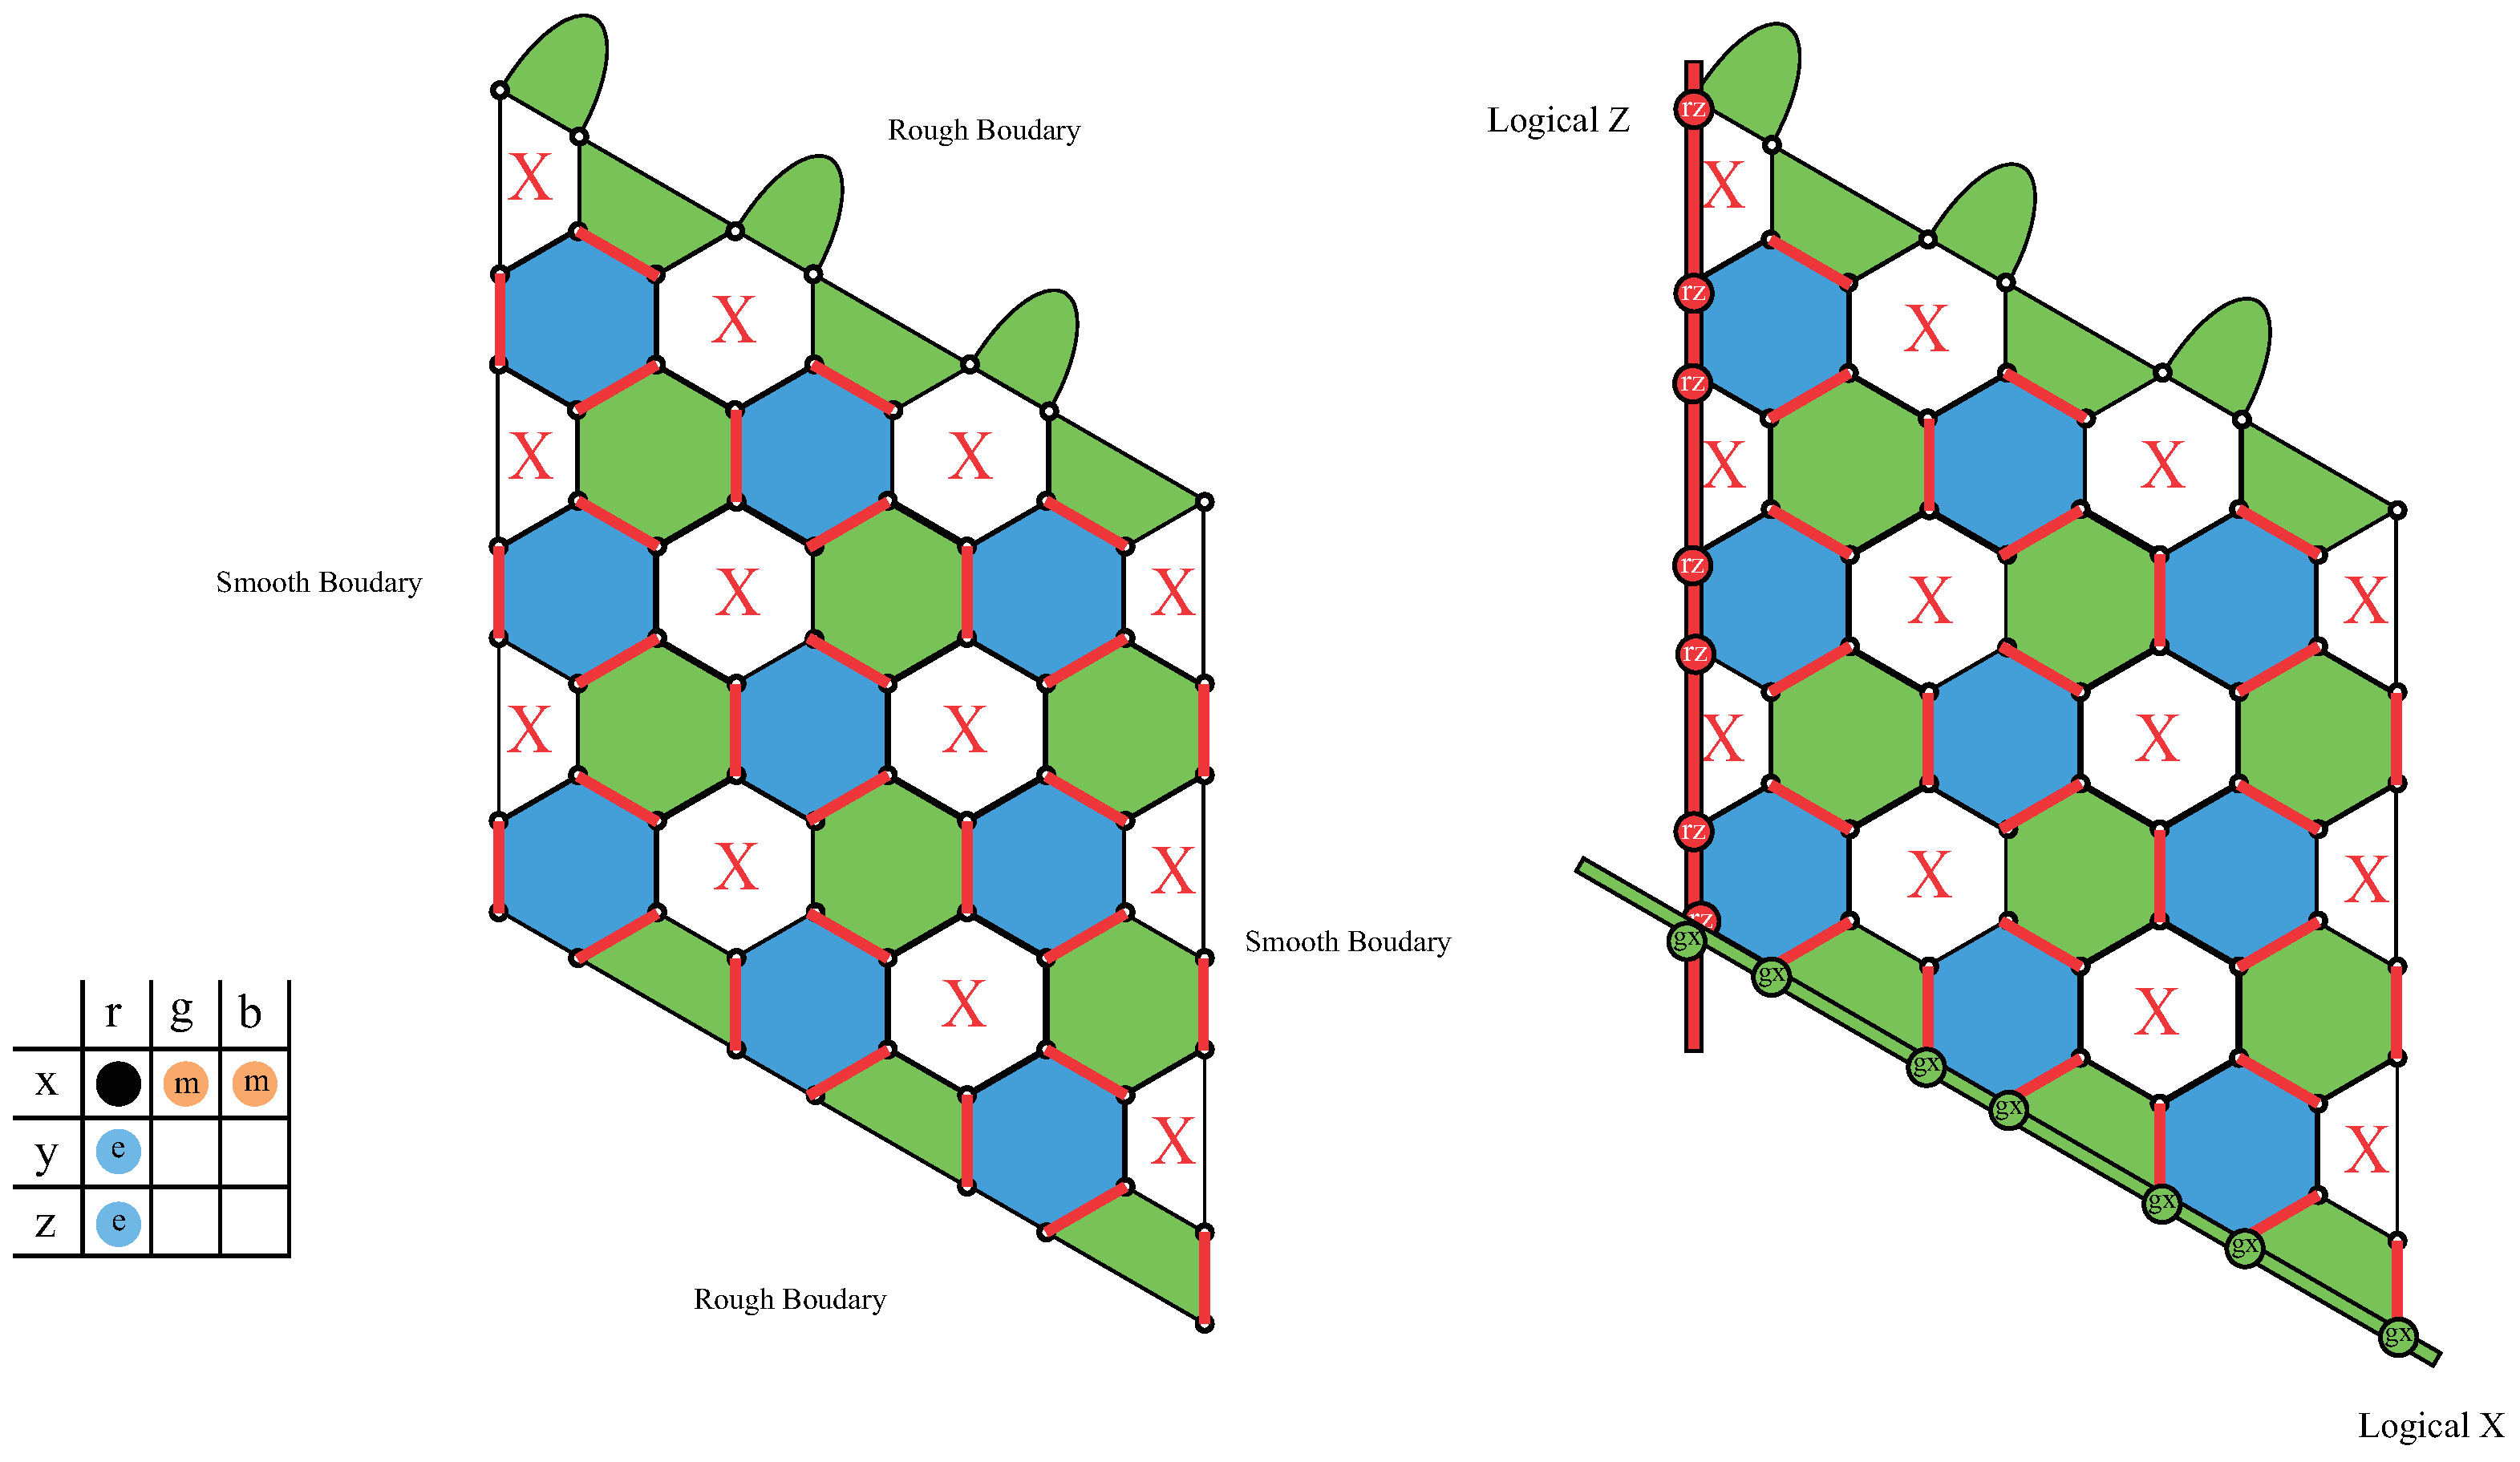
\includegraphics[scale=0.30]{figure/figure3.eps}
    \vspace{10pt}\caption{}
    \label{figure3}
    \vspace{-15pt}
  \end{figure}
  \clearpage
  Fig.4のように緑のZを選ぶ場合も同じグラフで実現することができる。Fig.3とFig.4ではanyon粒子を共有している部分があるためLogical Operatorを保存している。実際にグラフから確かめても、Logical Operatorは保存されている。赤Xから青Zへの変換も考えたが、うまく定義できなかった。
  \begin{figure}[h]
    \centering
    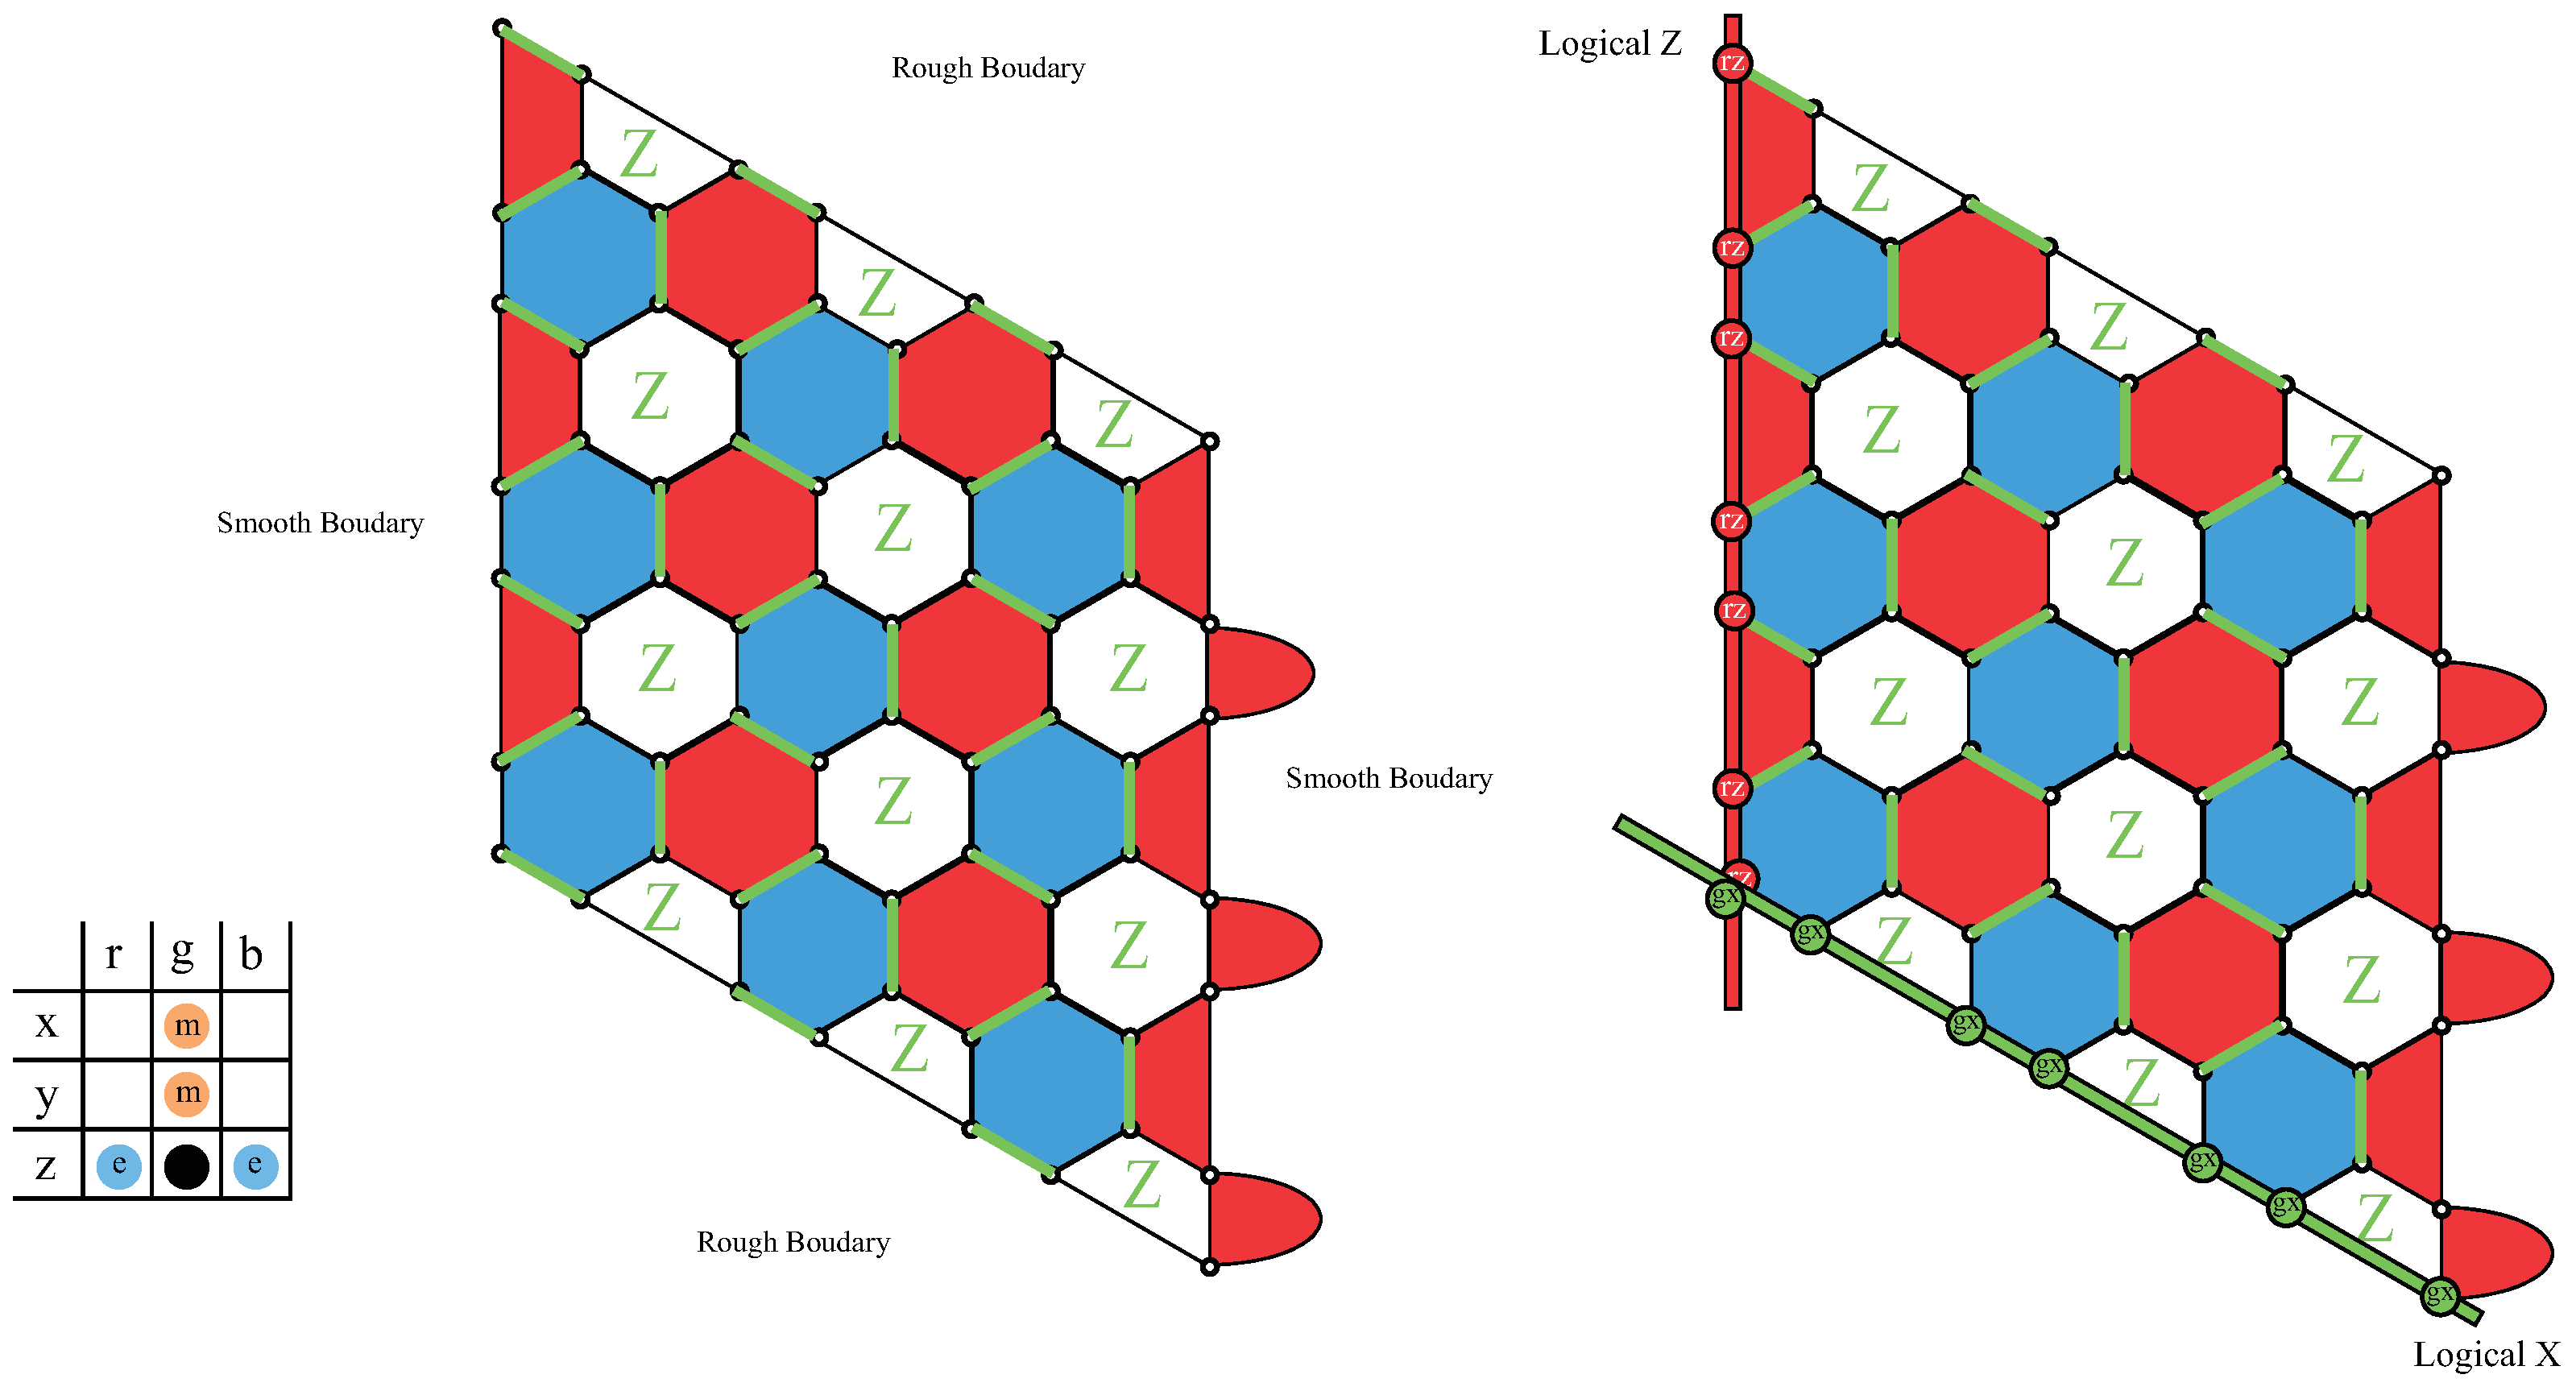
\includegraphics[scale=0.30]{figure/figure4.eps}
    \vspace{10pt}\caption{}
    \label{figure4}
    \vspace{-15pt}
  \end{figure}\\

\section{Unfolding Color Code}
   \cite{kubica2015}にCCをunitary transfomationすると、2つの重なったTCで表すことができることが示されている。このように実現されるCCはTCが折りたたまれたような構造になっている。\cite{gidney2024}でも指摘されているが、\cite{kubica2015}のunitary transformationでは符号距離が保存されない。また、そもそも計算の途中でunitary transfomationがどのように実行されるのかを私は理解していない。\cite{gidney2024}のescape stageでは、やむを得ずCCとTCのlattice surgeryを行って、符号距離を大きくしている。そこで、効率がいいのか全くわからないが、Floquet Color Codeの一つの例であるFig.3の符号を2つ使ってCCを実現し、Magic State Cultivationを行えると思う。最初から、2つのTCでCCを実現すれば、escape stageのgraftingが格段に楽になると思った。具体的には、以下のようなTCを用意する(Fig.5)。
  \begin{figure}[h]
    \centering
    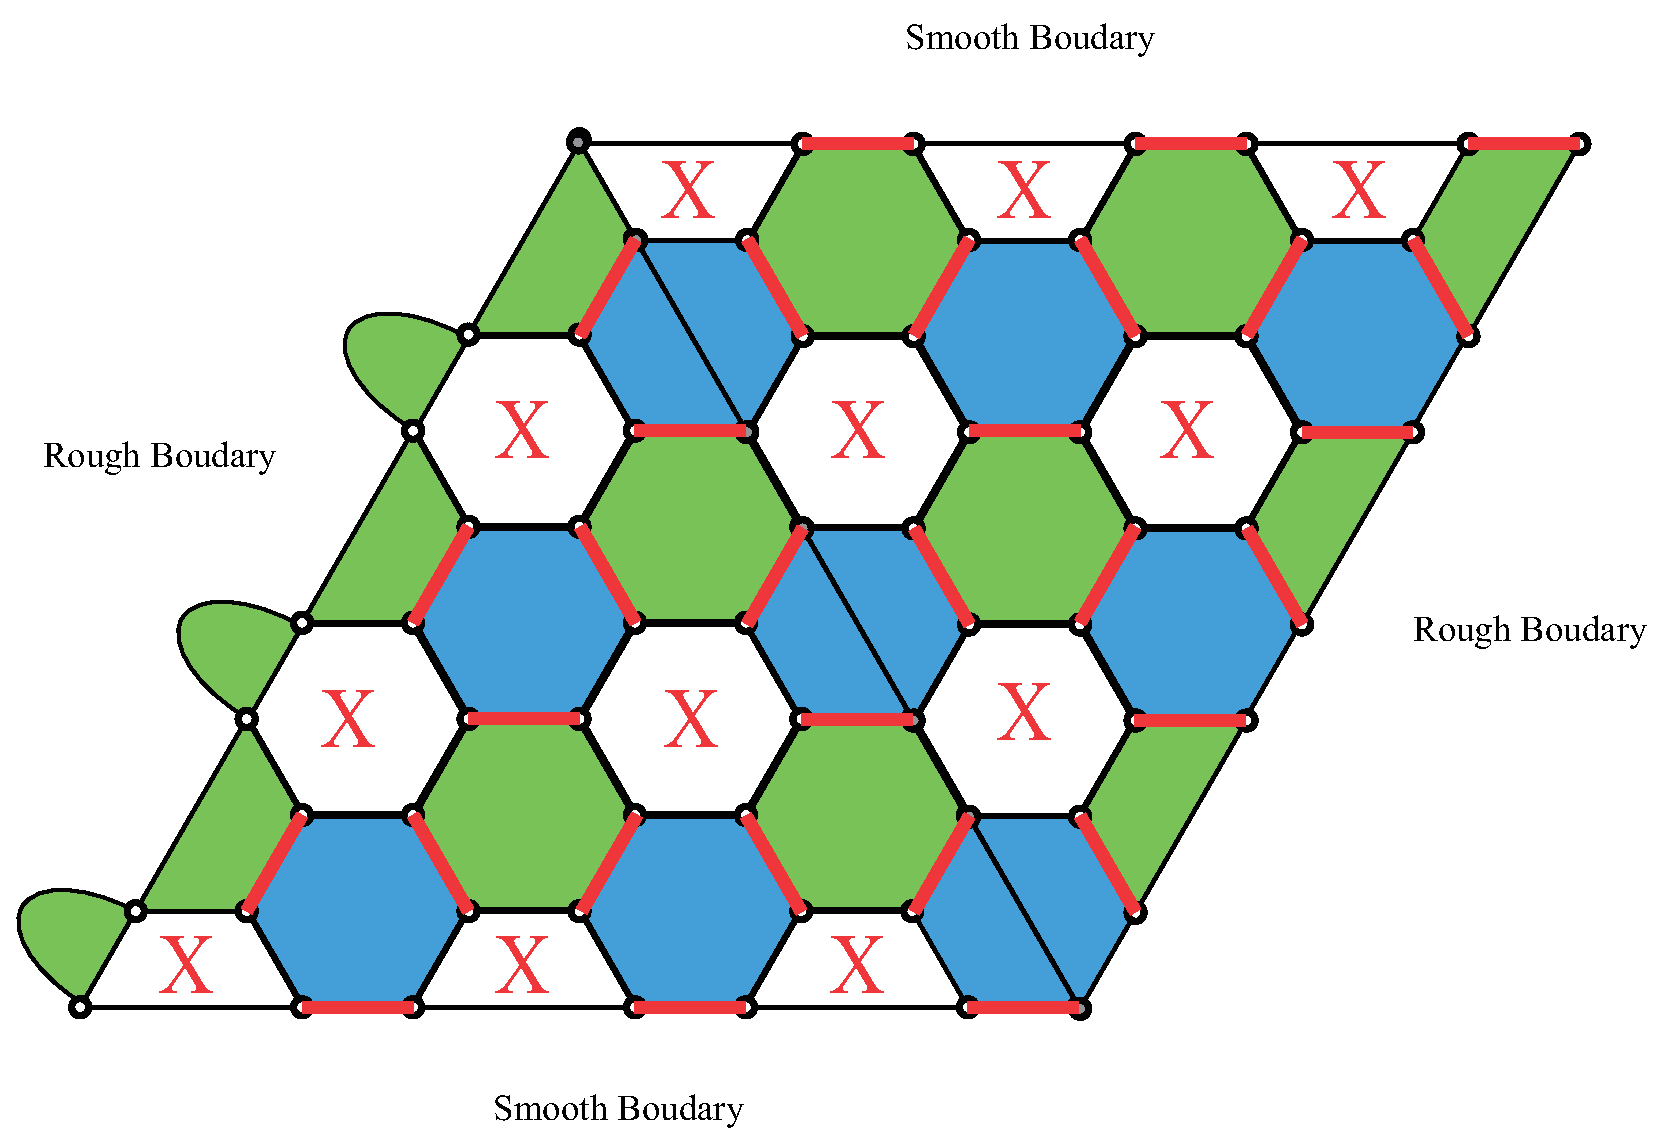
\includegraphics[scale=0.30]{figure/figure5.eps}
    \vspace{10pt}\caption{}
    \label{figure5}
    \vspace{-15pt}
  \end{figure}
  \clearpage
  Fig.5では平行四辺形の短い対角線が示されているがこれが折り目になっている。よって、CCを実現させるときはこの折り目で折りたたみ、Fig.6を作る。
  \begin{figure}[h]
    \centering
    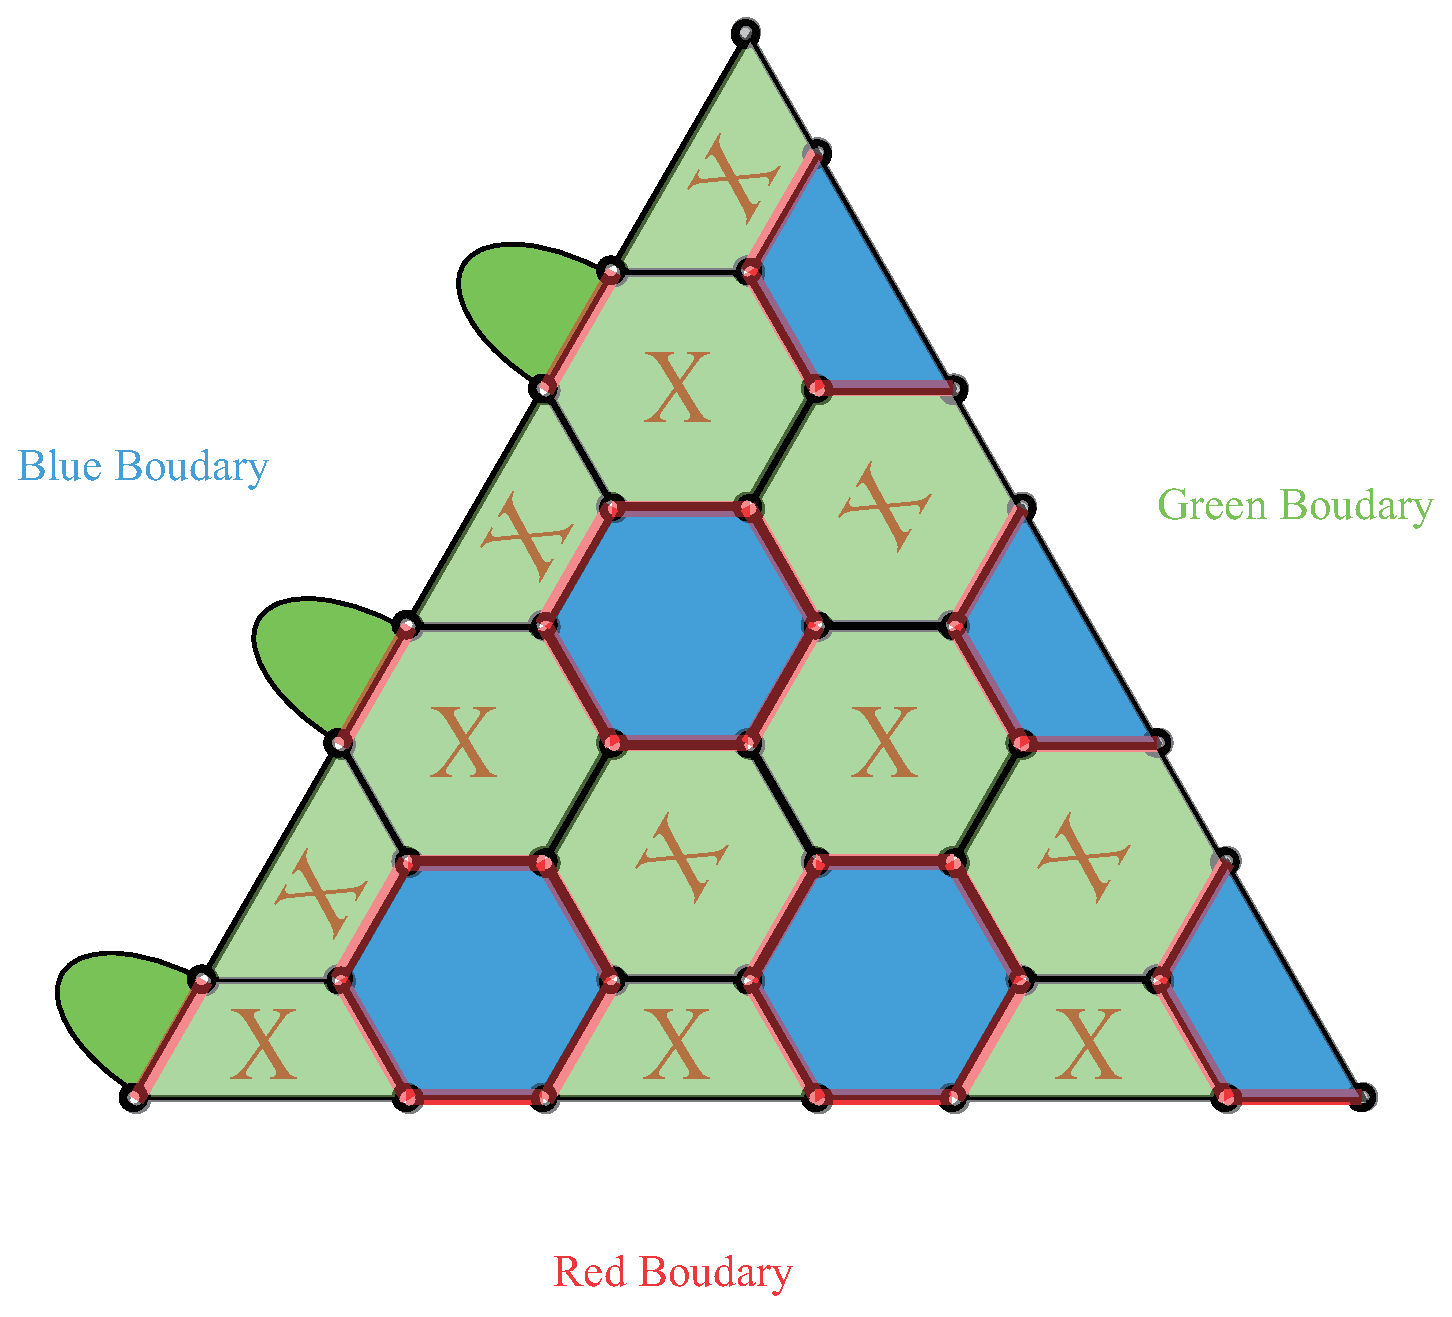
\includegraphics[scale=0.30]{figure/figure6.eps}
    \vspace{10pt}\caption{}
    \label{figure6}
    \vspace{-15pt}
  \end{figure}\\
  また、このときTCのanyon粒子を組み合わせて上げることで、CCのanyon modelを再現することができる。その組み合わせをTab.2に示す。ただし、添字の$+$は折りたたんだときの上のTC、$-$は折りたたんだときの下のTCを表す。また、$f=e\times m$である。
  \begin{table}[h]
    \centering
    \begin{tabular}{c|c|c|c}
       & r & g & b \\
      \hline
      x & $e^-$ & $e^-e^+$ & $e^+$ \\
      \hline
      y & $e^-m^+$ & $f^-f^+$ & $m^-e^+$ \\
      \hline
      z & $m^+$ & $m^-m^+$ & $m^-$ \\
      \hline
    \end{tabular}
    \caption{}
  \end{table}\\
  たしかにこのようにすることによって、condenseやconfineがCCと同じように起こることがわかる。そして、Lattice SurgeryはTCのLattice Surgeryと同じようにして行うことがおそらくできる。

\section{まとめ}
 今回示したFloquet Codeを折りたたむような方法を用いれば、Magic State Cultivationを効率よく行えるかもしれない。今回は3色でFloquet Codeを実装できてない(赤Xから青Zへの変換が思いつかない)ので\cite{kesselring2024}に示されている完全なFloquet Color Codeを実現できていない。Floquet Codeについて大して勉強したことがないので、途中で符号を変えることの利点をまだ理解していないが、それらを調査して、このような折りたたんだFloquet Color Codeに優位性があるのかないのかを確かめていきたい。
\printbibliography
\end{document}
